To test my claims, I measured the performance of the above operations in a real programming language and runtime. My computing environment consisted of a Windows 10 desktop with an Intel Core i5-4460T 1.90GHz Haswell processor. I used C\# 7.0 with the .NET Core 2.1.4 runtime. I used the excellent BenchmarkDotNet library to obtain performance metrics and plotted them with the R package ggplot2.

I compared the performance of a growth array implementation I had written in C\# to that of a heavily-optimized dynamic array provided by the C\# standard library, \texttt{System.Collections.Generic.List}. The \texttt{List} type had parameters $\VarInitCapacity = 4$ and $\VarGrowthFactor = 2$, while my growth array implementation had $\VarInitCapacity = 8$ and $\VarGrowthFactor = 2$. (The different values of $\VarInitCapacity$ were not significant since $\frac{8}{4}$ was a multiple of $\VarGrowthFactor$, causing the two collections to exhibit similar trends for large $n$.) I used 57 unique values of $n$ for the appending benchmarks, and 15 different values of $n$ for the other benchmarks. In both cases, input values included increasing powers of $2$ up to $32768$. For the appending benchmarks, I also tested with values of $n$ that were one more than a power of $2$, values that were the average of two consecutive powers of $2$, and values from $1$ to $10$. Here are my results:

\begin{figure}[H]
	\begin{minipage}{0.45\textwidth}
		\label{plot:1}
		\centering{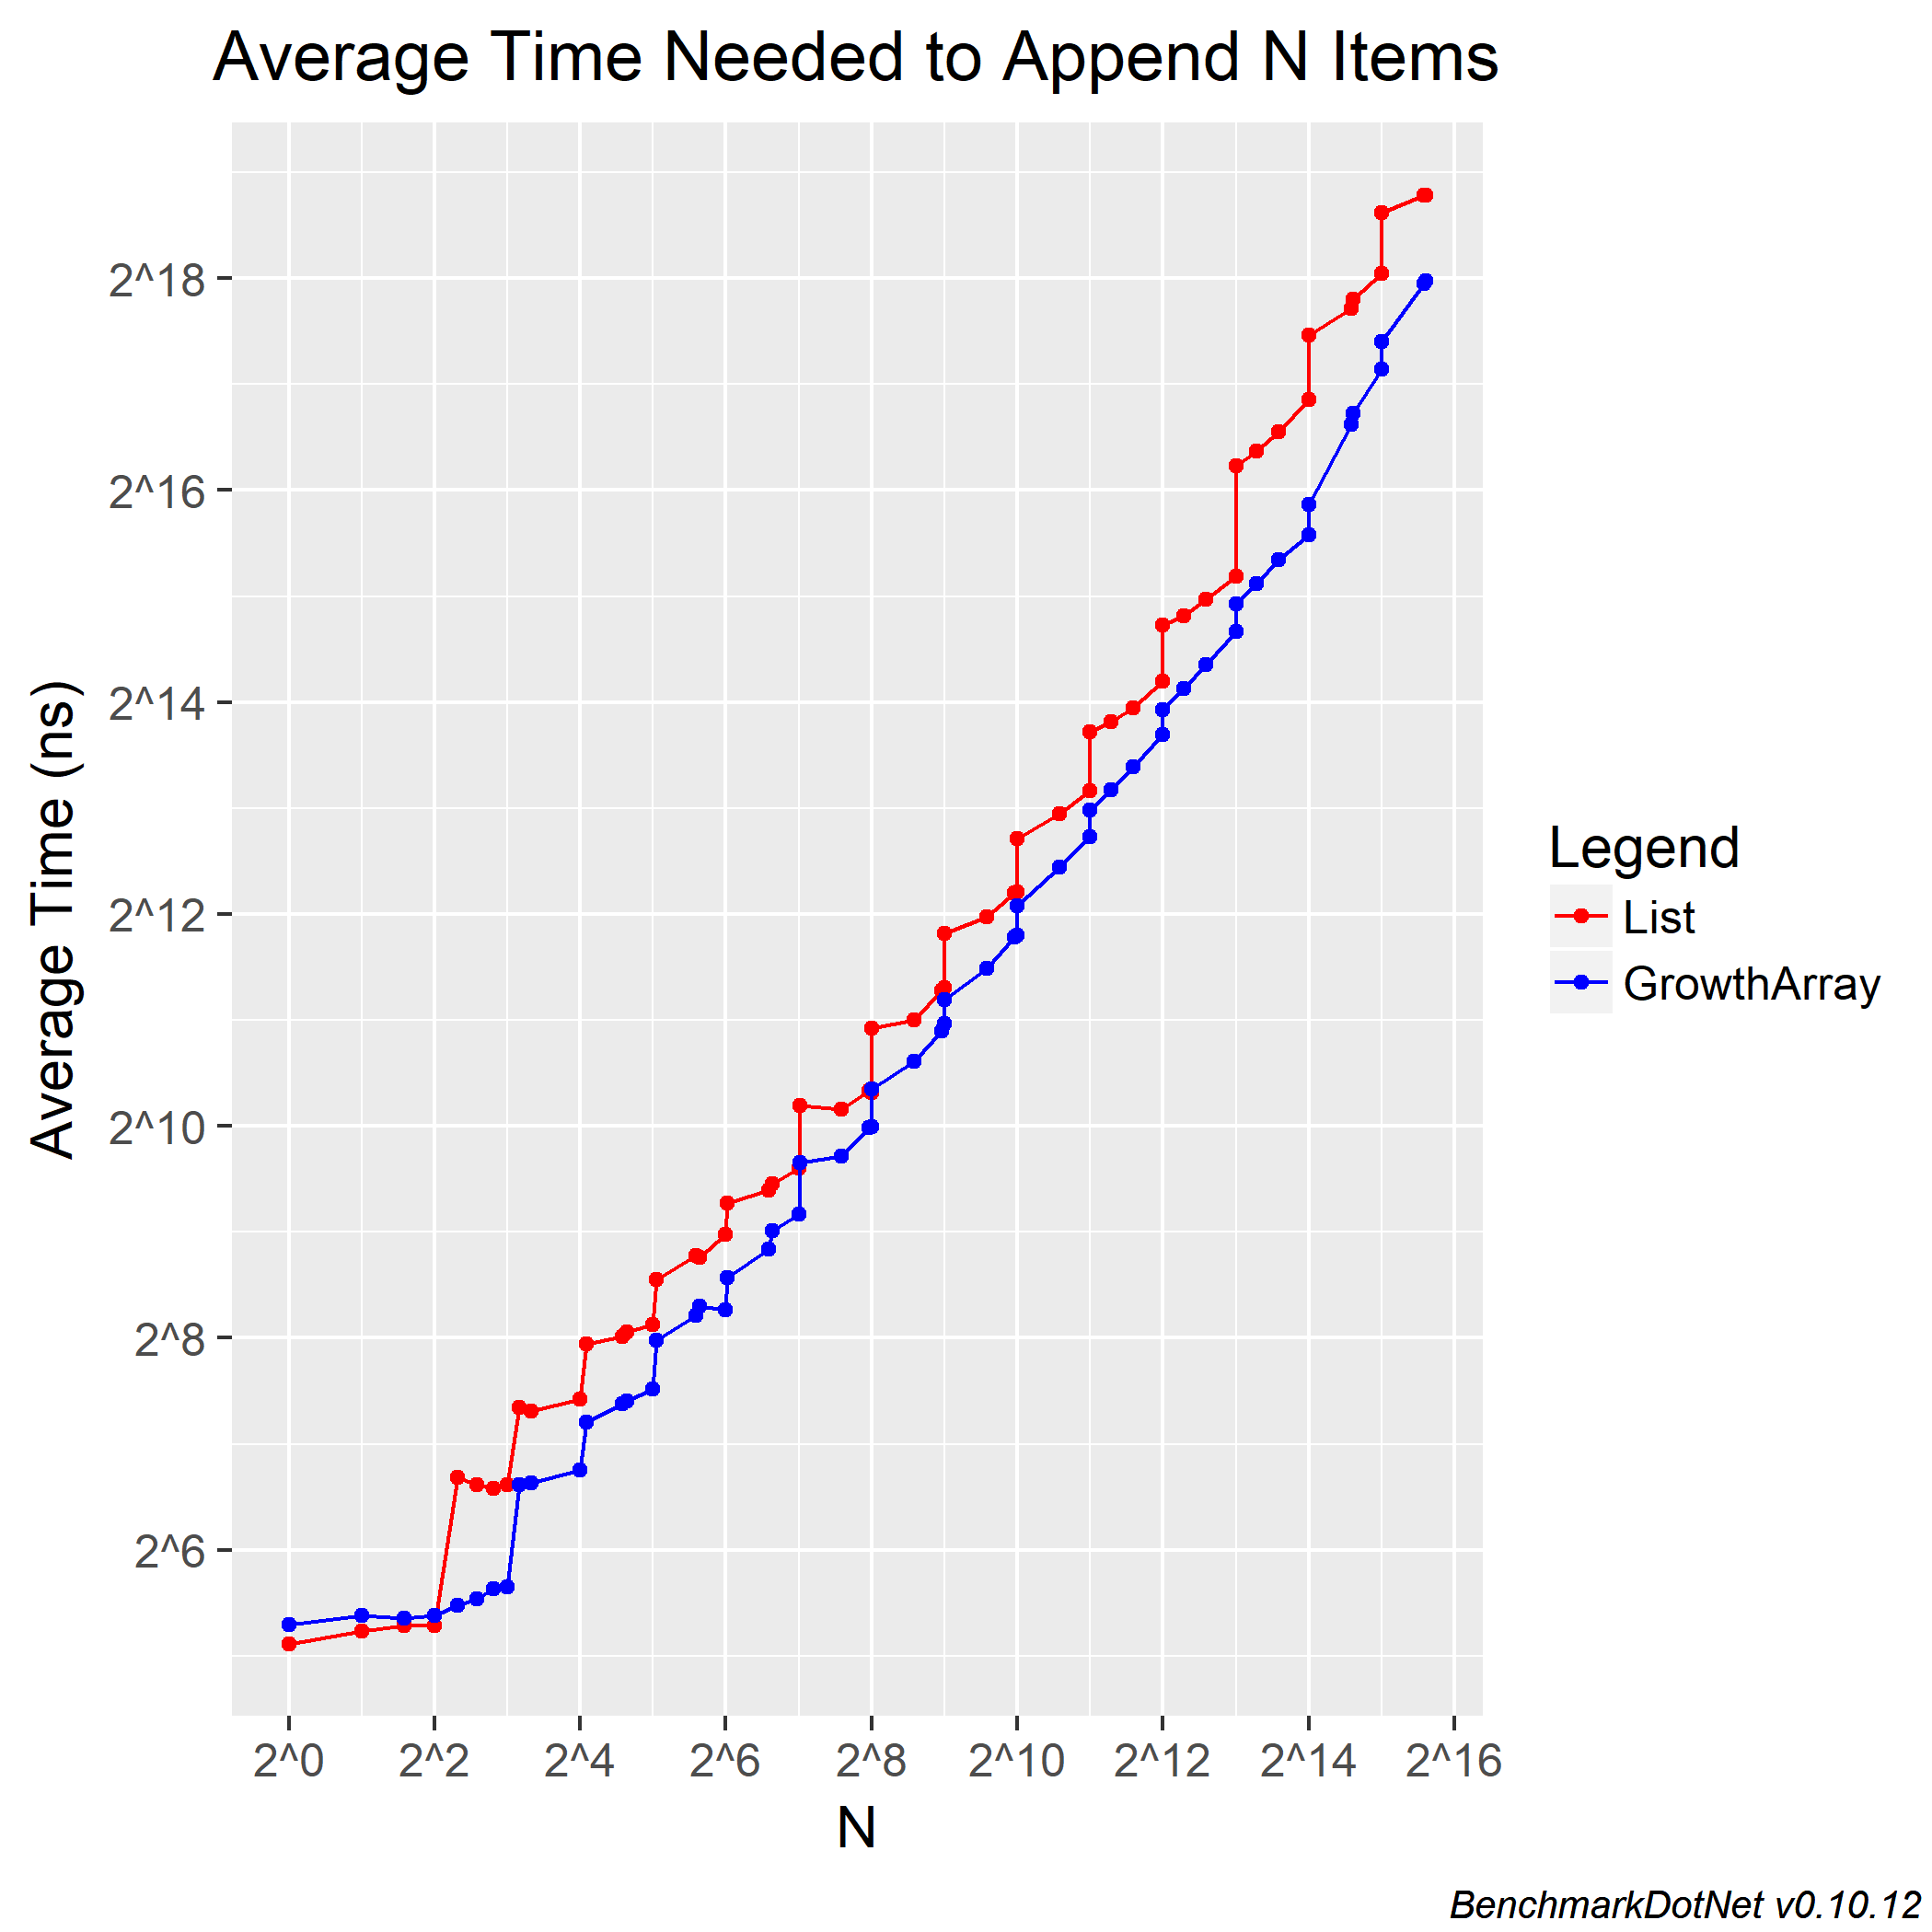
\includegraphics[width=3.25in]{Append-timeline}}
		\caption{Time measurements for appending}
	\end{minipage}\hfill
	\begin{minipage}{0.45\textwidth}
		\label{plot:2}
		\centering{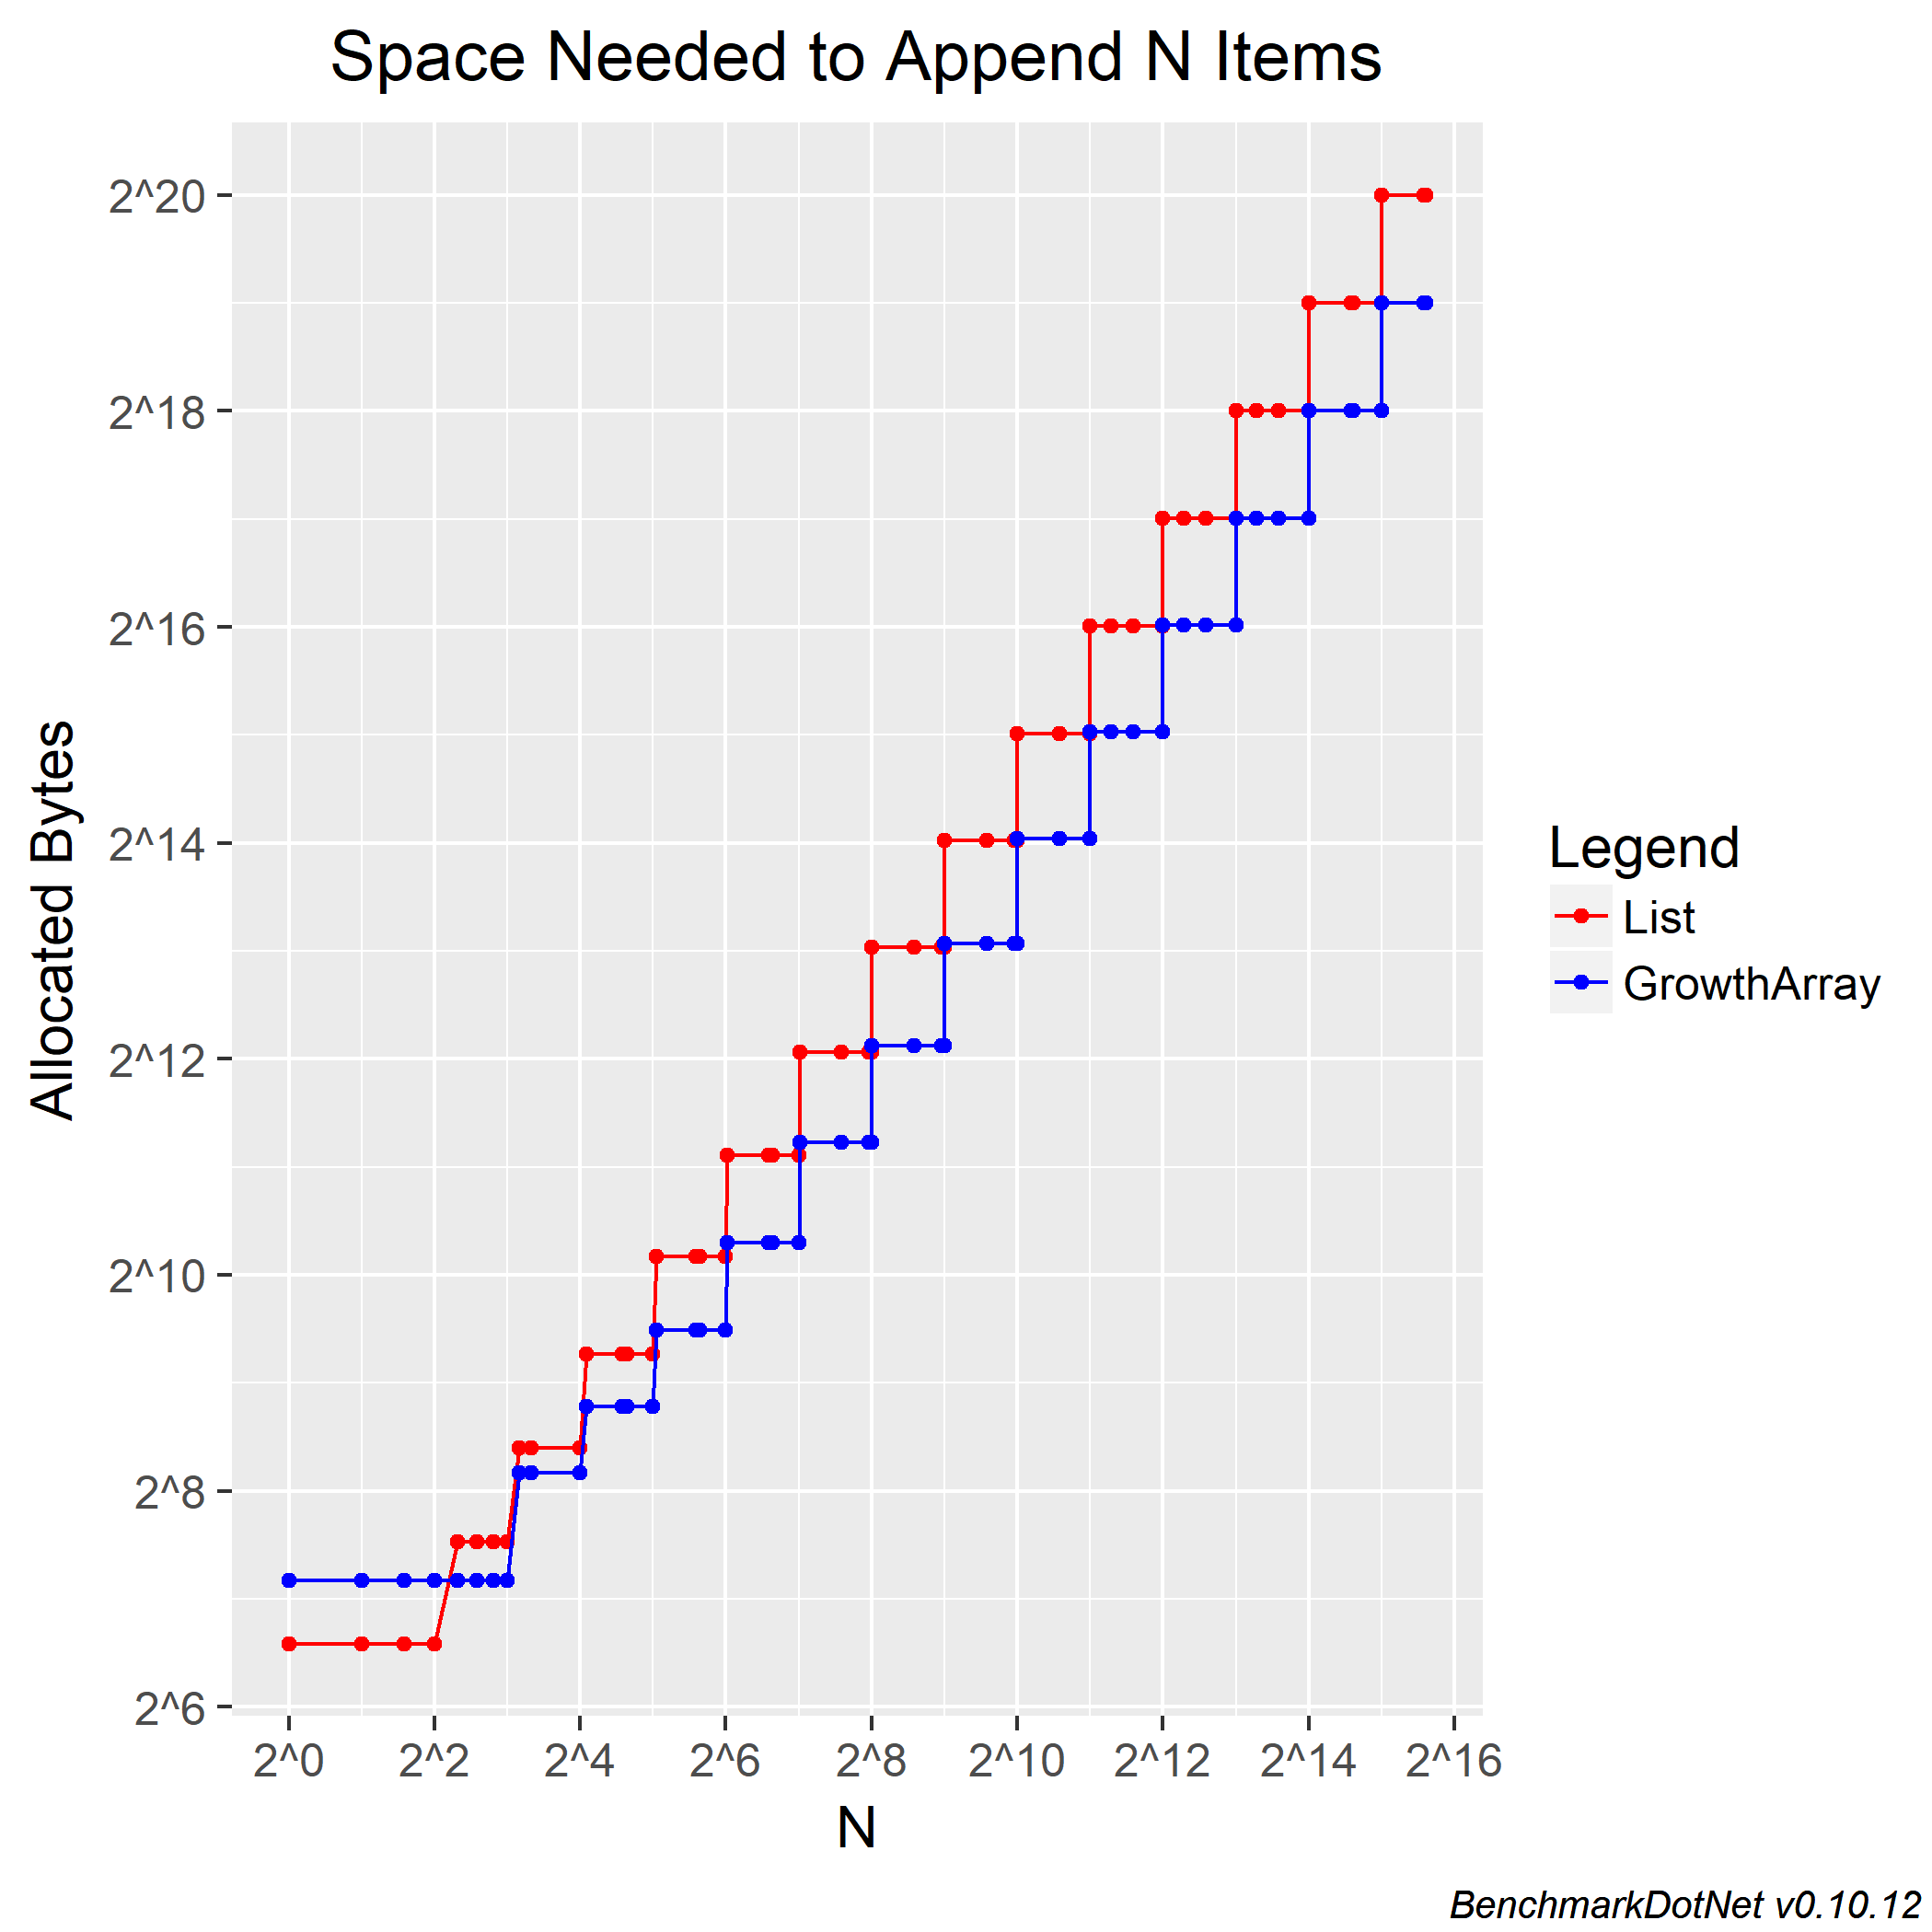
\includegraphics[width=3.25in]{Append-allocations}}
		\caption{Space measurements for appending}
	\end{minipage}
\end{figure}

\begin{figure}[H]
	\begin{minipage}{0.45\textwidth}
		\label{plot:3}
		\centering{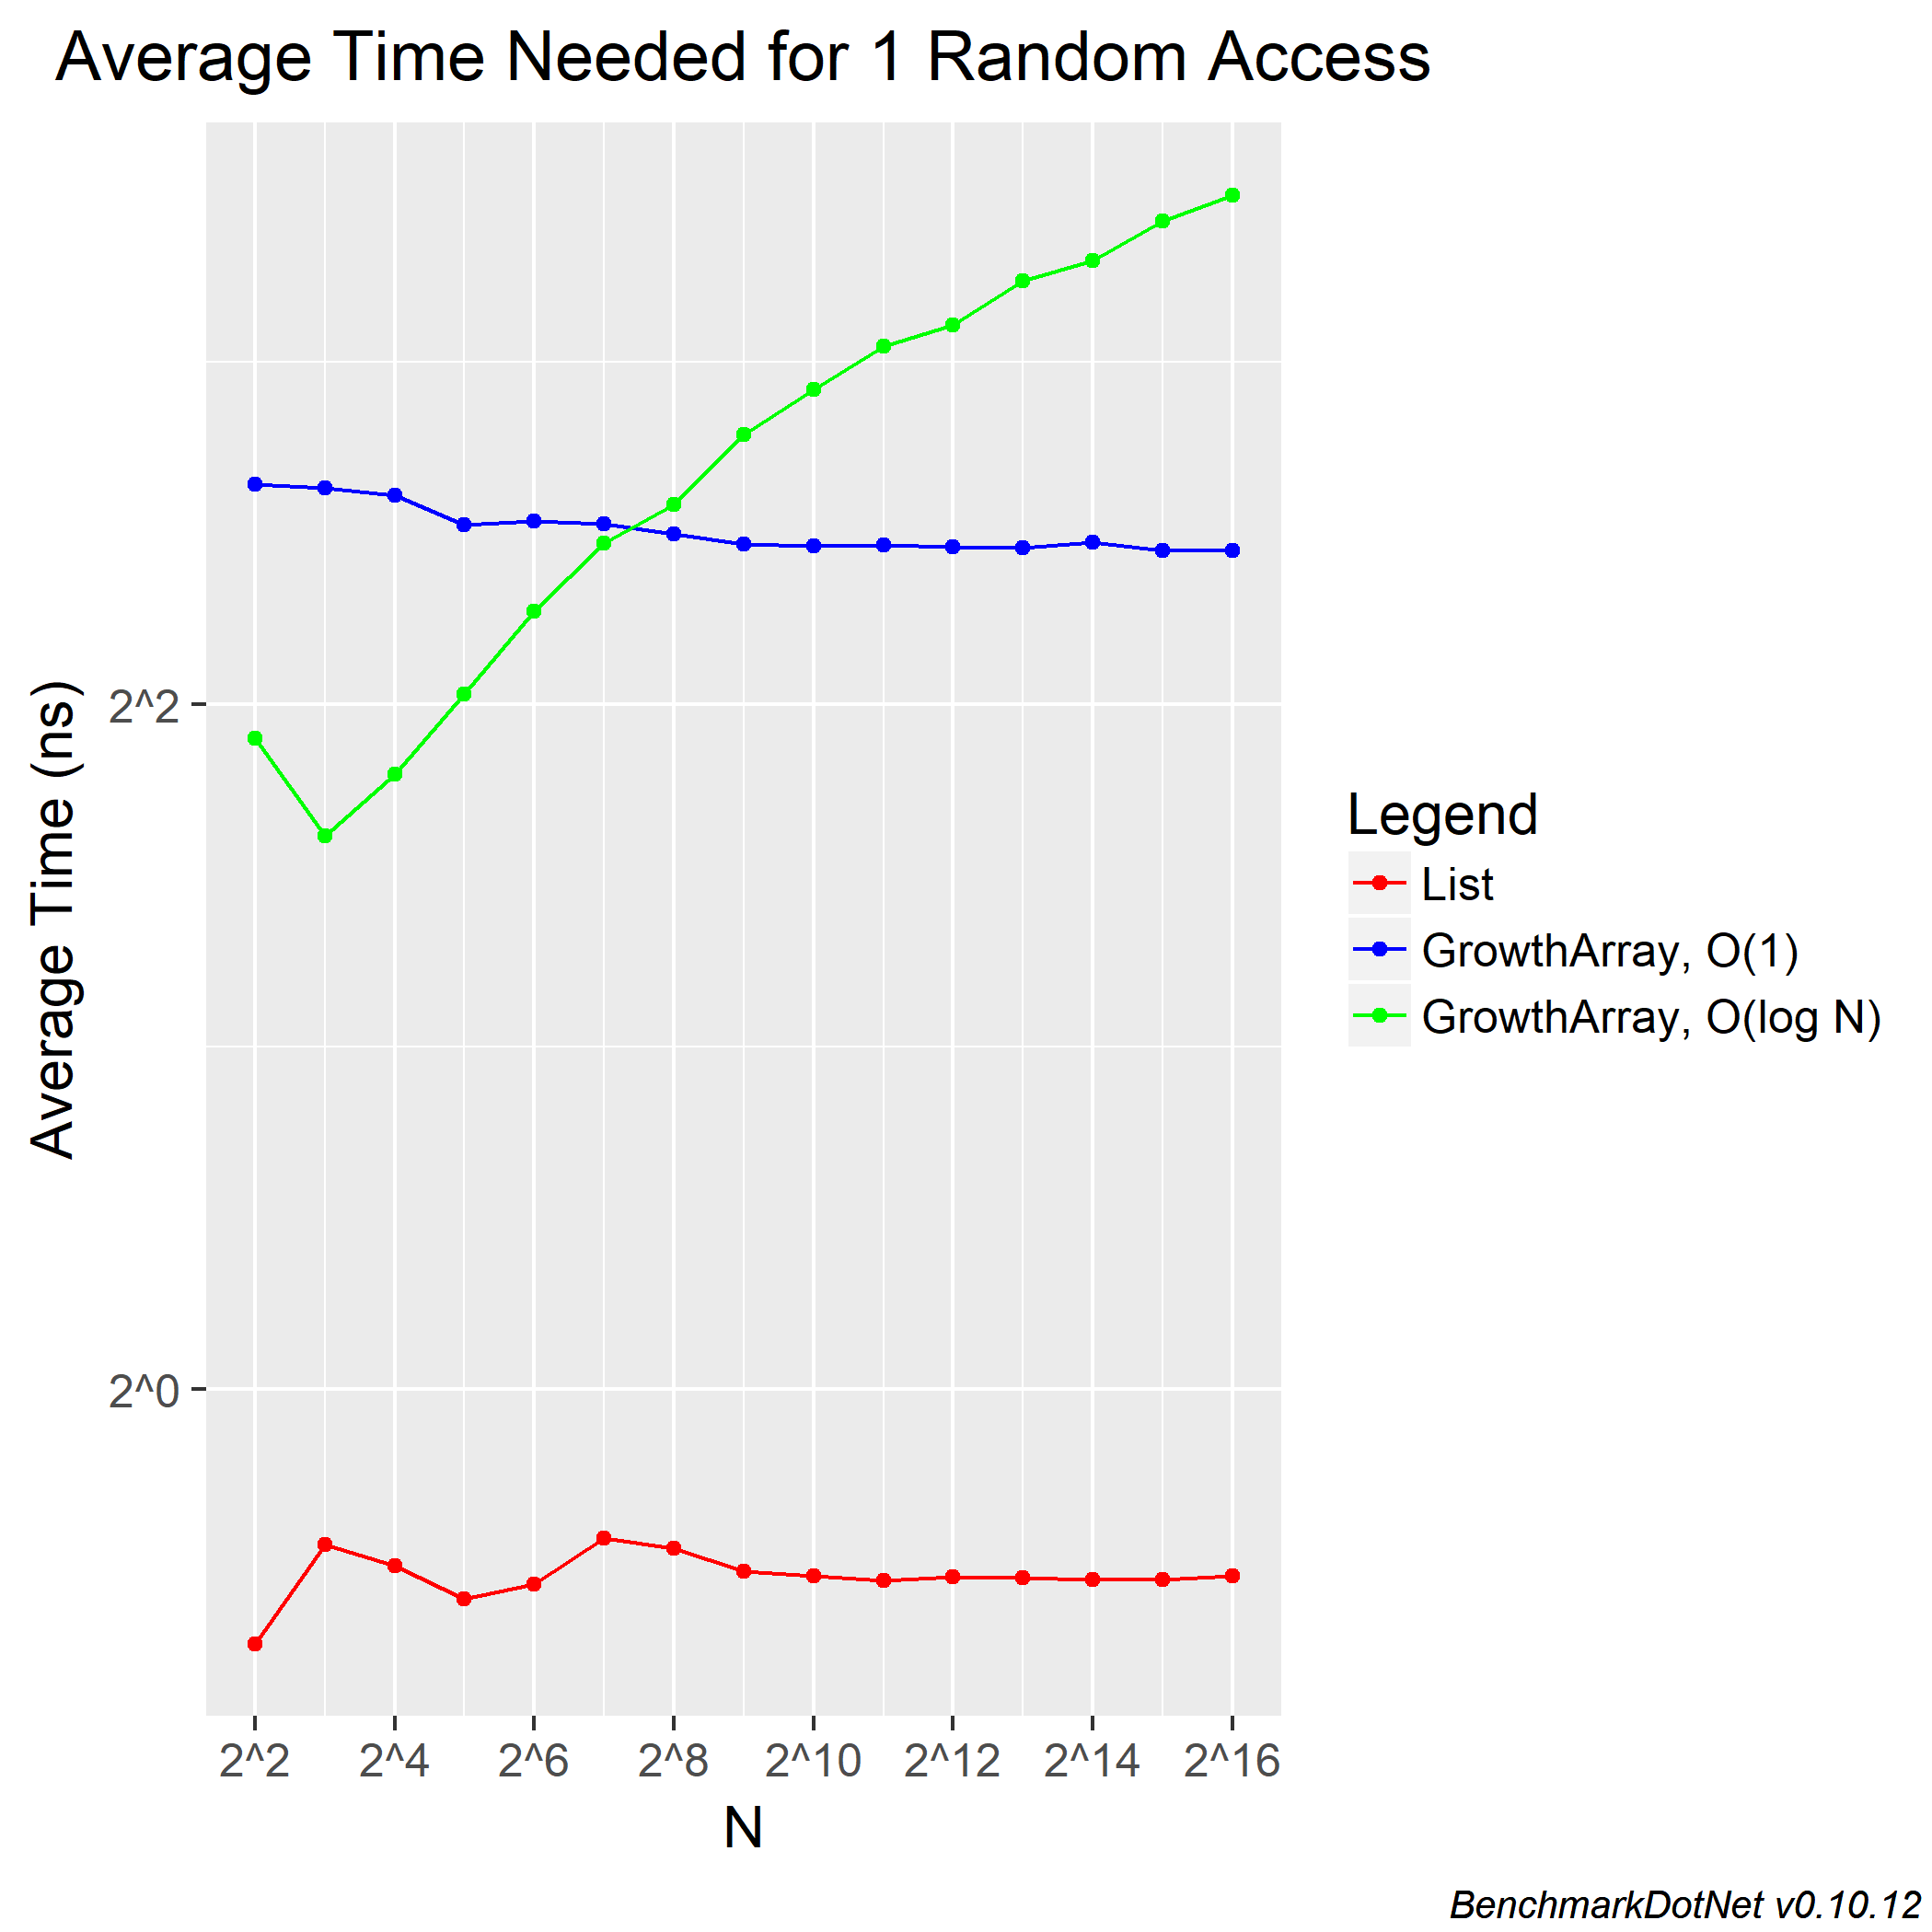
\includegraphics[width=3.25in]{GetItem-timeline}}
		\caption{Time measurements for indexing}
	\end{minipage}\hfill
	\begin{minipage}{0.45\textwidth}
		\label{plot:4}
		\centering{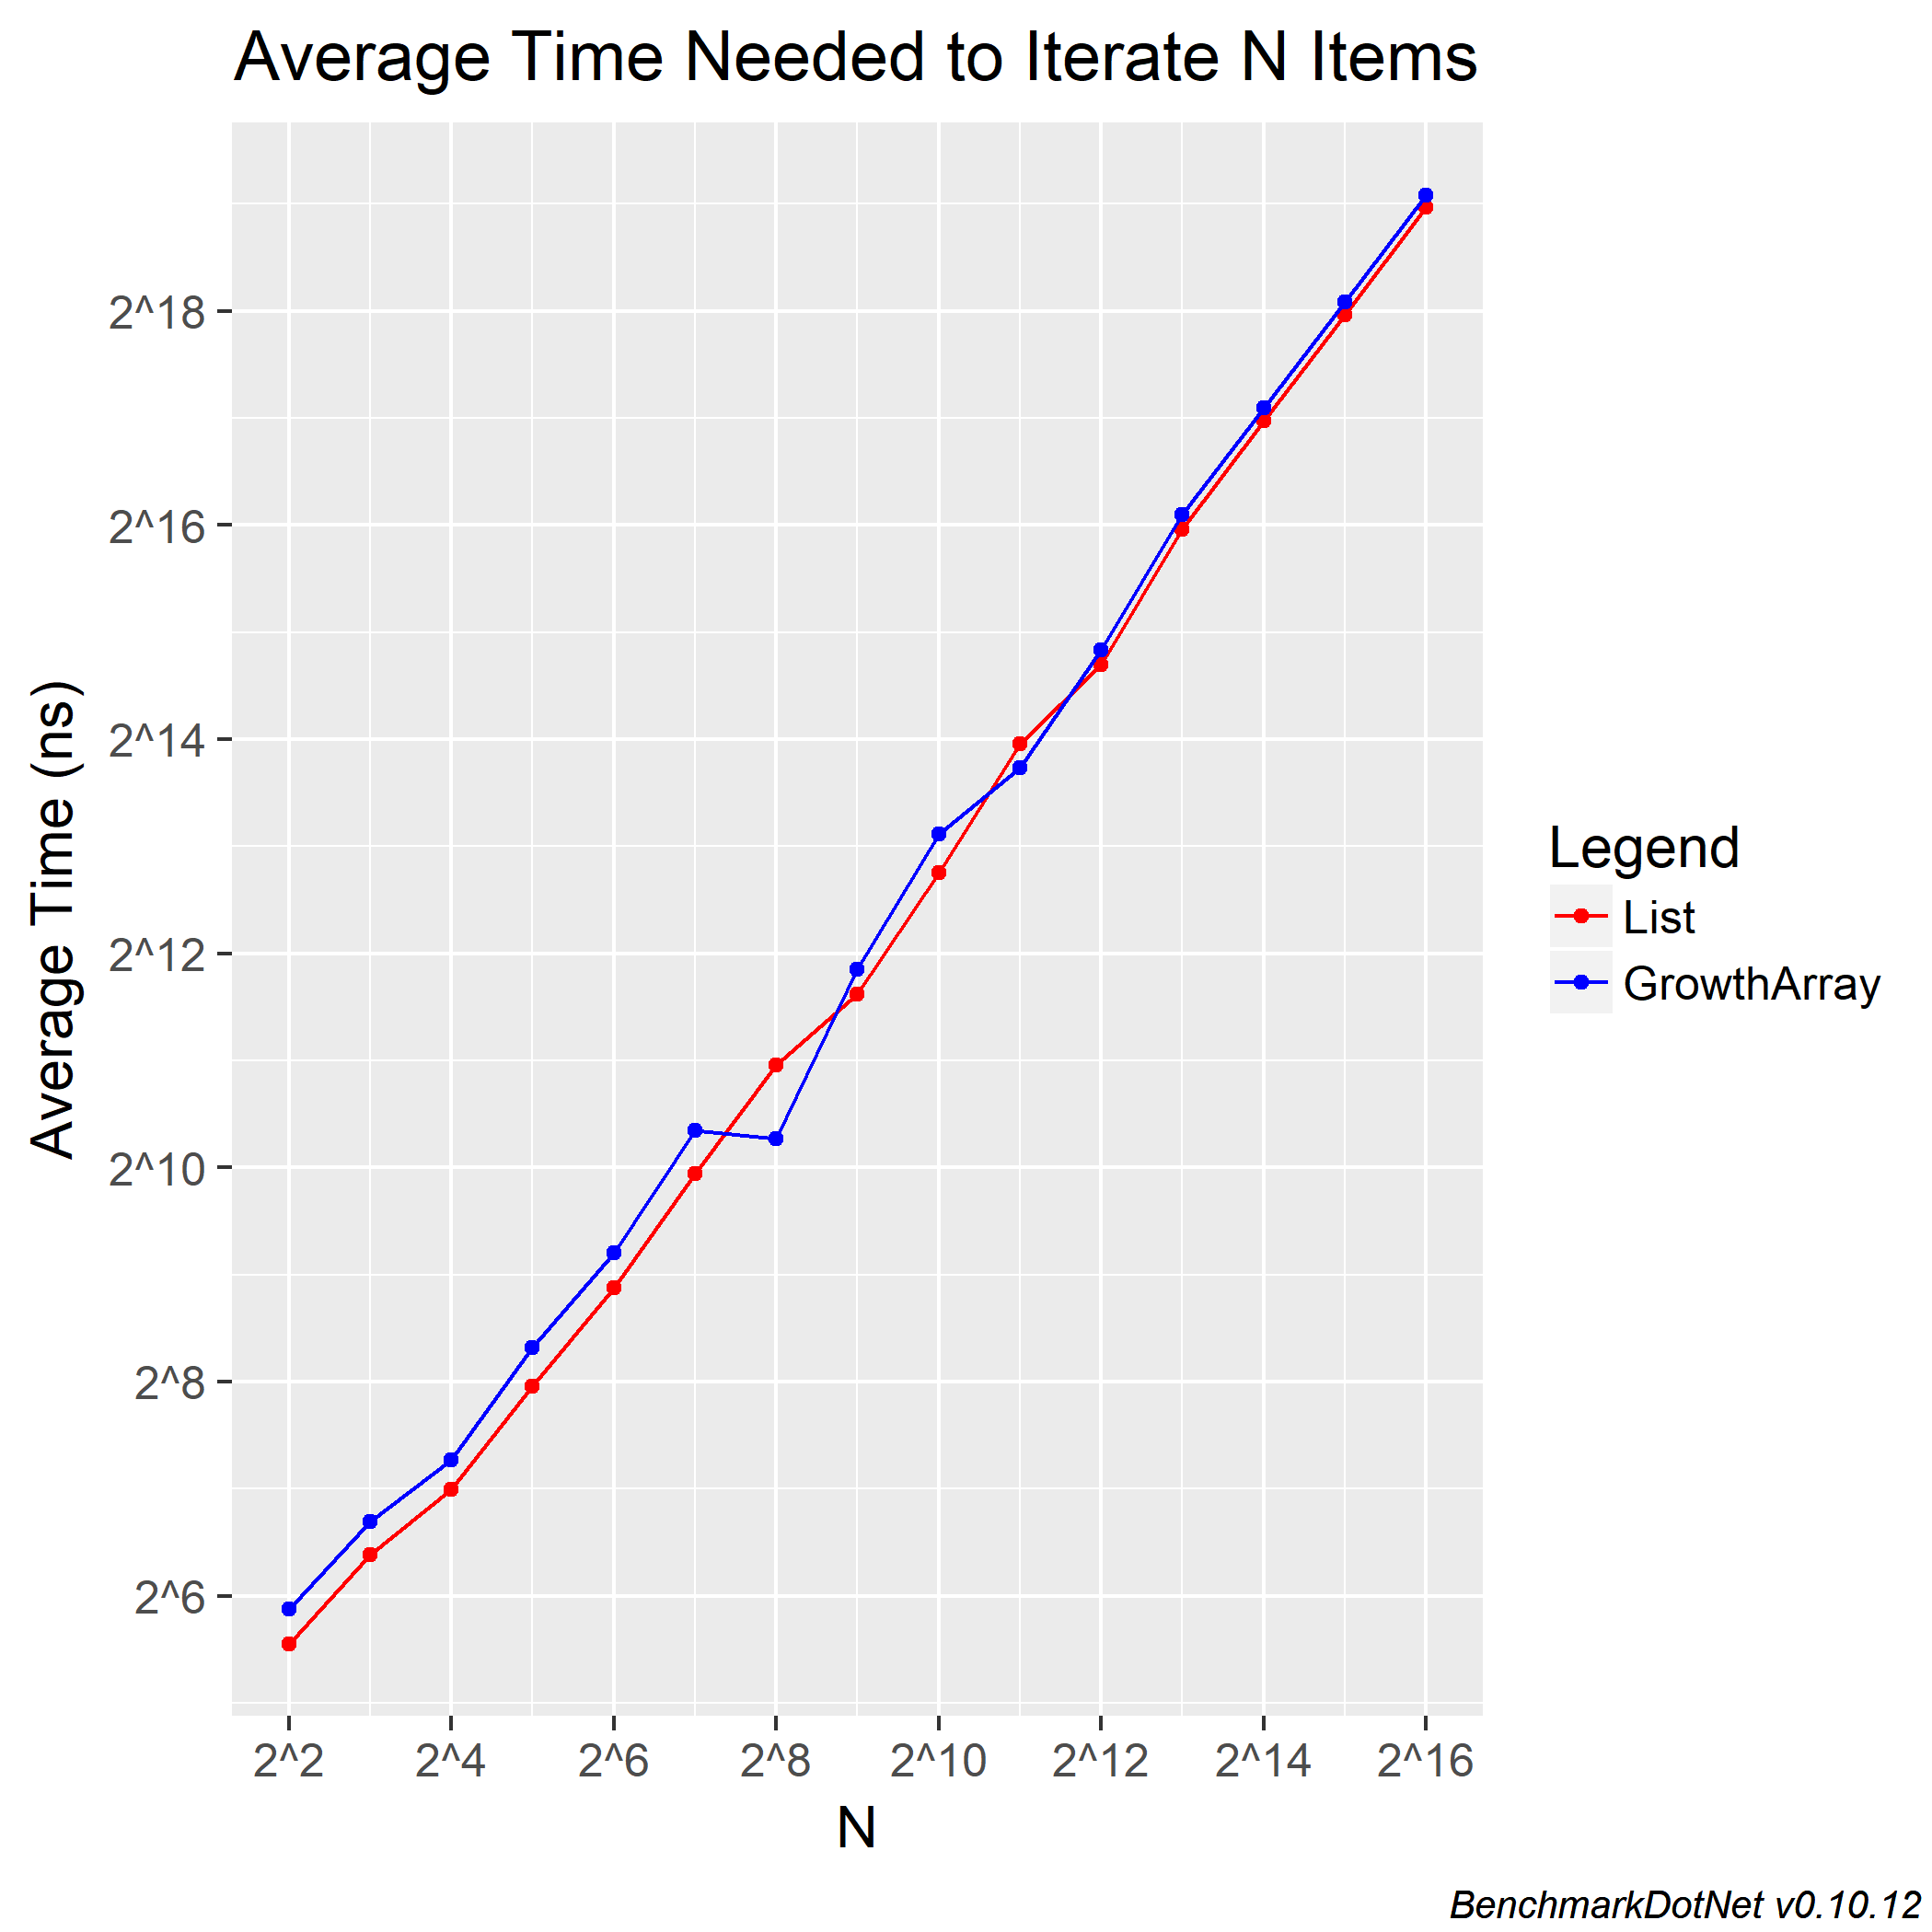
\includegraphics[width=3.25in]{Iteration-timeline}}
		\caption{Time measurements for iterating}
	\end{minipage}
\end{figure}

\begin{figure}[H]
	\begin{minipage}{\textwidth}
		\label{plot:5}
		\centering{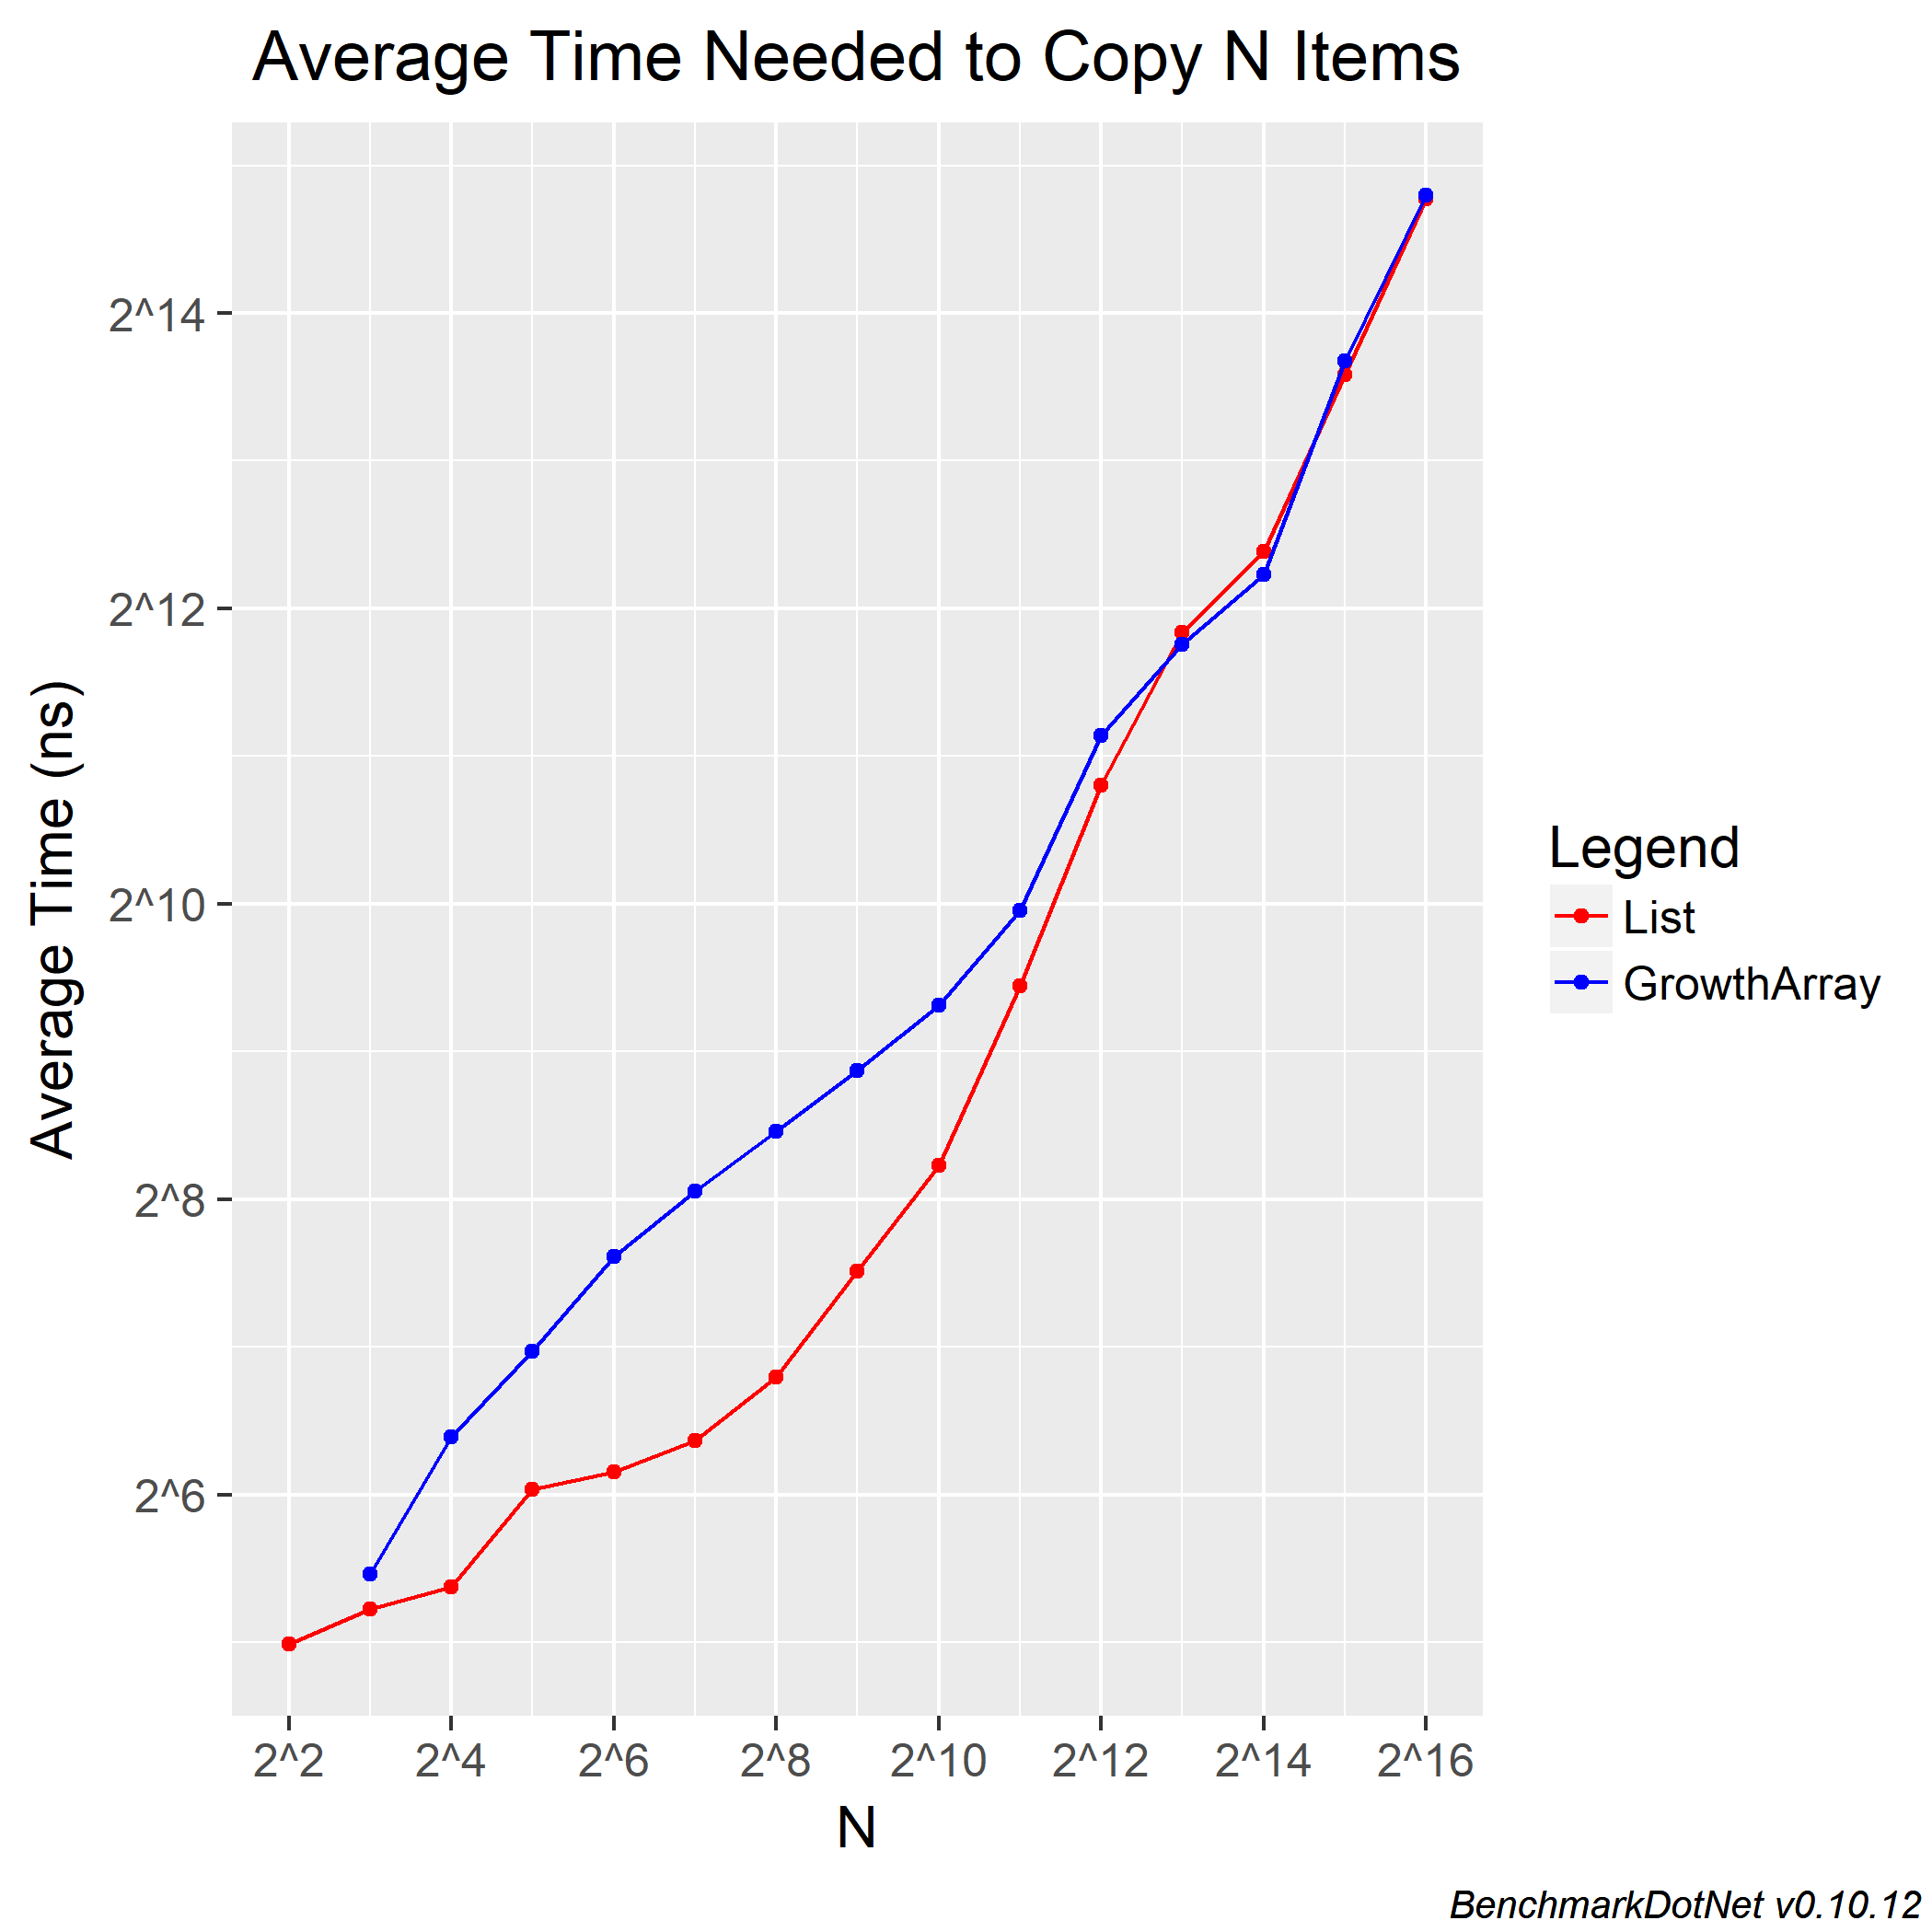
\includegraphics[width=3.25in]{Copying-timeline}}
		\caption{Time measurements for copying to raw arrays}
	\end{minipage}
\end{figure}

%% TODO: Why isn't \ref working?
Figures 4 and 5 show that growth arrays consistently outperform dynamic arrays at appending. Past $n = 4$, the blue line remains about one unit square below the red line for both graphs. Since the graphs are logarithmically scaled with one unit square representing a factor of $2$, I conclude that growth arrays use approximately half the time and half the space to append the same number of items as dynamic arrays for values of $n$ past $4$.

It misleadingly looks like the lines are touching for values of $n$ near powers of $2$. At these points, the blue and red lines appear to make vertical ``jumps.'' That is not what is really happening. The bottom end of each jump corresponds to when $n$ is a power of $2$, and the top end corresponds to when $n$ is one more than a power of $2$. The top end of each blue jump is close to the bottom end of each red jump, but it is incorrect to compare them since both points correspond to different values of $n$.

As you might guess, these jumps are where full capacity is reached and growth must occur. The sudden increase in time is mainly caused by the $O(n)$ memory allocation and (in dynamic arrays' case) the copying that happens when $\FuncGrow$ is called. Notice that the blue jumps are much less drastic than the red ones; this is because growth arrays do not make a copy of $n$ elements when they grow.

Figure 6 illustrates the graphs of 3 different random access algorithms, 2 of them for growth arrays. The constant time algorithms flat-line as they should, while the logarithmic time algorithm traces out a logarithmic curve. The dynamic array algorithm clearly beats both of the growth array algorithms: it appears to be approximately $8$ times faster than the constant time algorithm I introduced, and around $4$ times faster than the logarithmic time one at the point they are closest. An interesting observation is that the logarithmic time algorithm appears to outperform the blue constant time algorithm for values of $n$ that are $128$ or less.

Figures 7 and 8 show an interesting trend: the blue line converges towards the red line as $n$ gets very large. This supports the claim that I made in Sections \ref{subsec:Iterating} and \ref{subsec:ConvertRawArray} that not only do iteration and copying have the same time complexity for dynamic and growth arrays, their respective algorithms also have negligible time difference across data structures as $n$ gets very large. Also worth noting is the large gap that opens between the red and blue lines in Figure 8 for values of $n$ between $8$ and $4096$. This suggests that for small values of $n$, the extra overhead growth arrays introduce by iterating the tail's buffers is very significant.

For all benchmarks, BenchmarkDotNet consistently reported margins of error and standard deviation values on the order of $\frac{1}{100}$th of the measurement values.
